\problemname{Jogging Tour}

You may know that in the 17th century, a group of Dutchmen founded a settlement called New Amsterdam on Manhattan Island that later went on to become New York City.
Less well-known is the story of another group of Dutchmen that also moved over to America and founded a city called \emph{New Delft}.
Like its bigger counterpart, New Delft has been built on a grid made up of two sets of parallel streets that meet each other at a perpendicular angle.

Some stroopwafel bakeries have already been built in New Delft, but none of the streets have been constructed.
Your task is to lay out the grid of streets.
For this, you need to decide on an orientation for the grid so that there are two orthogonal directions for the two types of streets.
Once the orientation is fixed, you may build arbitrary streets, as long as each of them has one of the two given directions, as shown in Figure~\ref{fig:tour}.
Each street can be traversed in either direction.

\begin{figure}[!h]
  \centering
  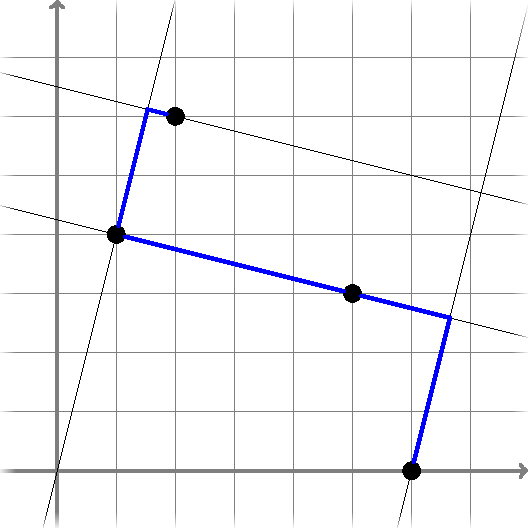
\includegraphics[width=0.4\textwidth]{sample2.pdf}
  \caption{Illustration of Sample Input 2 with a possible street layout that gives the shortest possible path that visits all bakeries in some order.}
  \label{fig:tour}
\end{figure}

The street layout should be created in an optimal way for the annual \emph{Stroopwafel Run}.
This is an event in which a group of runners visits all the bakeries in some order of their choosing, and they may start and end their run at any point in the city.
Your task is to come up with a grid layout that makes this shortest path as short as possible.

\begin{Input}
  The input consists of:
  \begin{itemize}
    \item One line with an integer $n$ ($2 \le n \le 12$), the number of stroopwafel bakeries in New Delft.
    \item $n$ lines, each with two integers $x$ and $y$ ($0 \le x,y \le 10^6$), the coordinates of one of the bakeries.
  \end{itemize}
  The bakeries are at distinct coordinates, so for any $1 \le i,j \le n$ with $i \neq j$, it holds that $(x_i, y_i) \neq (x_j, y_j)$.
\end{Input}

\begin{Output}
  Output the length of the shortest possible path that visits all bakeries in some order, assuming an optimal grid layout.

  Your answer should have an absolute or relative error of at most $10^{-6}$.
\end{Output}
